 
\ChapterWithAuthor{Căutare binară}{Andrei-Cristian Ivan}

\section{Problema inițială}
Să presupunem că avem un șir de $N$ numere și memorie astfel încât să putem reține \textit{doar} șirul (plus evident alte variabile, dar nu foarte multe). Noi primim mai multe întrebări, de forma: Există valoarea $X$ în șir?

În mod evident, o soluție foarte trivială este să parcurgem manual șirul pentru fiecare întrebare, și să vedem dacă elementul cerut apare sau nu în șir, astfel obținând complexitate totală de \O{N \cdot Q}. Singura noastră problemă este că noi o să avem $N$ și $Q$ undeva în jur de $10^6$, ceea ce va face ca această abordare să pice clar în timp, deci va trebui găsită o soluție mult mai eficientă. Aici intervine algoritmul de \textit{căutare binară}.

\section{Prezentarea algoritmului}
\textbf{Notă:}\ De acum încolo, se va presupune că șirul nostru este sortat crescător. Căutarea binară pe un șir nesortat va da mereu răspunsuri eronate.

În algoritmul de căutare binară se va pleca de la analiza șirului pe întreaga sa lungime, și se va fixa punctul de mijloc din sir. Dacă valoarea poziției din mijloc este mai mică decât valoarea căutată, atunci sigur valoarea căutată se poate (că nu știm sigur dacă există!) afla în a doua jumătate, altfel, se poate afla în prima jumătate. Mai departe, nu va mai fi necesar sa analizăm tot șirul, ci doar jumătatea relevantă (cea în care considerăm noi că există o șansă să găsim valoarea noastră), și algoritmul se va repeta până când lungimea devine $1$ și putem determina răspunsul. Dat fiind faptul că noi la fiecare pas împărțim la $2$ lungimea șirului, acest lucru ne va da complexitate logaritmică la determinarea răspunsului, deci vom avea complexitate \O{Q \log N} (dacă șirul nostru nu este sortat din input, se mai adaugă și un \O{N \log N} la complexitate), cu memorie \O{N}.

Pentru o înțelegere mai clară a algoritmului, să presupunem următorul exemplu: se dă un șir sortat crescător unde apar toate numerele de la $1$ la $100$, și se cere să determinăm dacă există în șir valoarea $72$.

\begin{center}
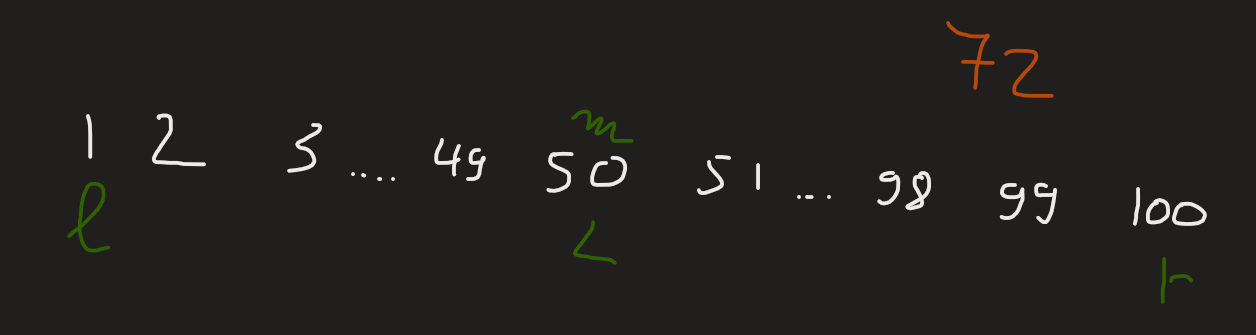
\includegraphics[width=\textwidth]{images/cautari/cb1.png}
%\vspace{0.12cm}
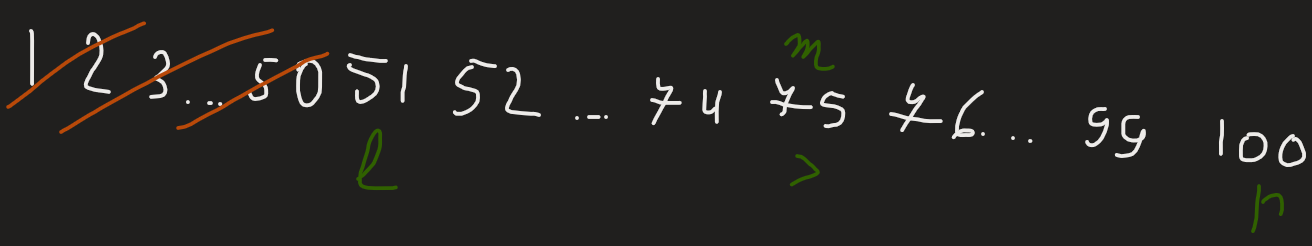
\includegraphics[width=\textwidth]{images/cautari/cb2.png}
%\vspace{0.12cm}

\includegraphics[width=\textwidth]{images/cautari/cb3.png}
%\vspace{0.10cm}
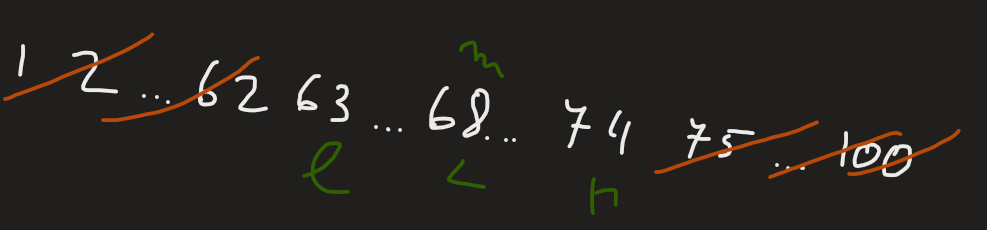
\includegraphics[width=\textwidth]{images/cautari/cb4.png}
%\vspace{0.10cm}
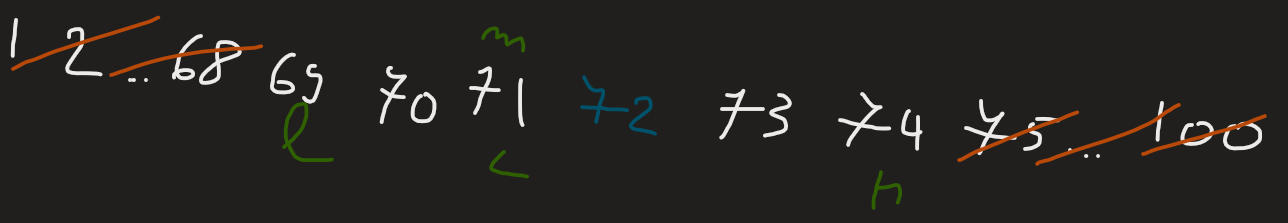
\includegraphics[width=\textwidth]{images/cautari/cb5.png}
%\vspace{0.10cm}

\includegraphics[width=\textwidth]{images/cautari/cb6.png}
%\vspace{0.05cm}

\includegraphics[width=\textwidth]{images/cautari/cb7.png}
%\vspace{0.05cm}
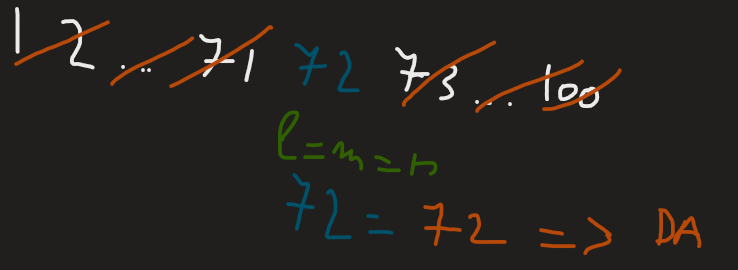
\includegraphics[width=\textwidth]{images/cautari/cb8.png}
\end{center}

O întrebare la care trebuie totuși dat răspuns este: De ce împărțim în două jumătăți și de ce nu în $3$ treimi? Da, $\log_3 N < \log_2 N$, dar numărul de verificări efectuate va fi mai mare la împărțirea în $3$ treimi, deci în continuare este mai eficient să împărțim în două jumătăți. În mod inductiv se va demonstra pentru orice împărțire posibilă.

\section{O implementare banală}
Cea mai des întâlnită implementare a căutării binare este următoarea:
\cpp{codes/cautari/cb1.cpp}

Implementarea de mai sus este una corectă, dar se pot întâlni următoarele bug-uri:
\begin{itemize}
    \item Schimbarea în $\equals{l}{mij}$ și $\equals{r}{mij}$ va face ca programul nostru să ruleze într-o buclă infinită (deoarece ambele valori vor atinge la un moment dat valoarea $mij$, și deci va fi respectată mereu condiția $l \leq r$)
    \item În timp ce-l calculăm pe $mij$, ne putem lua overflow (dacă prin absurd ajungem să căutam fix pe la valorile maxime pe care le poate reține tipul nostru de date, este inevitabil un overflow generat de $l + r$). De aceea, următoarea variantă prezentată se va axa fix pe rezolvarea acestui bug.
\end{itemize}

\section{O implementare corectă}
\cpp{codes/cautari/cb2.cpp}

Această căutare binară se bazează pe principiul menționat mai sus: noi înjumătățim de fiecare dată lungimea șirului pe care încercăm să căutăm ceea ce ne interesează. Formula de mai sus pentru calcularea mijlocului este echivalentă cu cea din prima căutare, dar mai mult, nu are cum să ne dea overflow.

De fiecare dată când mijlocul nostru verifică \emph{condiție}, noi facem un \emph{„salt”} de la o poziție $l$ la alta. La finalul căutării, indicele $l$ final va fi defapt o sumă a salturilor, iar ca pe orice număr întreg, noi acest număr îl putem descompune într-o altă bază numerică. Hai să vedem cum putem rafina această idee cu o altă implementare mai jos.

\section{Căutarea binară a lui Mihai Pătrașcu}
\cpp{codes/cautari/cb3.cpp}

Baza în care noi vom descompune suma va fi baza $2$, pentru a menține în continuare complexitatea $\log_2 N$. Inițial, vom pleca cu un exponent $e$, unde $2^e$ va reprezenta lungimea secvenței pe care o analizăm (atenție să nu ieșim din vector!). Chiar dacă noi vom analiza inițial o lungime care este putere de $2$, care foarte probabil să fie diferită de $N$, se poate demonstra foarte ușor că noi (dacă o să fie necesar), vom putea căuta valori și în acea secvență neacoperită inițial. Lăsăm această demonstrație ca temă pentru cititor.

Căutarea de mai sus poartă și numele de \emph{Căutarea binară a lui \href{http://people.csail.mit.edu/mip/}{Mihai Pătrașcu}}, sau \emph{căutarea pe biți}.

În mare parte, aceste căutări binare ne vor da aceeași complexitate peste tot, în schimb, când vrem să implementăm algoritmul de Lowest Common Ancestor (LCA) cu Binary Lifting, căutarea binară pe biți reduce algoritmul de la \O{\log^2{H}} la \O{\log{H}}, unde $H$ reprezintă adâncimea maximă a arborelui.

\section{Concluzii și lecturi suplimentare}

Căutarea binară este unul dintre cele mai fundamentale principii ale algoritmicii, fiind absolut necesar pentru a optimiza probleme unde ni se cere să determinăm existența unei valori într-un șir, sau determinarea unui număr maxim / minim care să respecte o condiție impusă de problemă etc.

Pentru aprofundarea a algoritmului, recomand rezolvarea următoarelor probleme și citirea următoarelor articole:

\begin{itemize}
    \item \href{https://www.infoarena.ro/problema/cautbin}{Problema cautbin (Infoarena)}
    % \item \href{}{}
    % \item \href{}{}
\end{itemize}
